\documentclass[a4paper]{article}
\usepackage[utf8]{inputenc}
\usepackage[german]{babel}
\usepackage{graphicx}

\author{Alin Porcic}
\title{DVB - Digital Video Broadcast}

\begin{document}

\maketitle
\newpage

\section{DVB}

\subsection{Allgemeines}

DVB steht für "Digital Video Broadcast'' und beschreibt ein standardisiertes Verfahren zur Übertragung von digitales Fernsehen. Durch aufwendige Datenkompression (z.B. MPEG-4) können digitale Inhalte im Gegensatz zum analogen Fernsehen durch höhere Datenkompression mehr Programme pro Sendekanal übertragen werden. 

\subsection{Übertragungsmedien}

\begin{itemize}
\item \textbf{DVB-S} $\rightarrow$ für die Übertragung durch direkt strahlende Satelliten 
\item \textbf{DVB-S2} $\rightarrow$ aktueller Nachfolgestandard für DVB-S
\item \textbf{DVB-C} $\rightarrow$ für die Übertragung über Kabelnetze
\item \textbf{DVB-C2} $\rightarrow$ Nachfolger des DVB-C
\item \textbf{DVB-T} $\rightarrow$ für die Übertragung durch terrestrische Senderketten im VHF- bzw. UHF-Bereich
\item \textbf{DVB-T2} $\rightarrow$ Nachfolger des DVB-T Standards
\item \textbf{DVB-H} $\rightarrow$ für die asynchrone Übertragung auf mobile Endgeräte, ebenfalls terrestrisch
\item \textbf{DVB-IPI} $\rightarrow$ für die Übertragung über IP-basierende Netzwerke, zum Beispiel Internet (Internet Protocol Infrastructure)
\item \textbf{DVB-RC(S/C/T)} $\rightarrow$ Rückkanal (Return Channel) für die Übertragung von Datendiensten, zum Beispiel Breitbandinternet
\item \textbf{DVB-SI} $\rightarrow$ für die Übertragung der Service Information
\item \textbf{DVB-SH} $\rightarrow$ für die Übertragung über Satellit auf mobile Endgeräte
\end{itemize}

\subsection{Unterschiede der Übertragung}

Das Übertragungsverfahren kann bei den verschiedenen Übertragungsmedien des DVB unterschiedlich variieren. Hier ist eine kurze Zusammenfassung der Übertragung der verschiedenen Medien:

\begin{itemize}

	\item \textbf{DVB-S (Satellit)} $\rightarrow$ \begin{itemize}
	\item Modulationsart: QPSK
	\item Übertragungskapazität: typsich 33Mbit/s bis 38Mbit/s
	\item Empfang: Parabolantenne 
	\item Mobilität: stationär, bedingt tragbar (mobil)
	\end{itemize}
	
	\item \textbf{DVB-S2 (Satellit, HDTV)} $\rightarrow$ \begin{itemize}
	\item Modulationsart: QPSK, 8PSK, 16APSK oder 32APSK
	\end{itemize}	
	
	\item \textbf{DVB-C (Kabel)} $\rightarrow$ \begin{itemize}
	\item Modulationsart: 16 bis 256 QAM
	\item Übertragungskapazität: typsich 38Mbit/s (64 QAM)
	\item Mobilität: stationär
	\end{itemize}

	\item \textbf{DVB-C2 (Kable)} $\rightarrow$ \begin{itemize}
	\item Modulationsart: 16 bis 256 QAM
	\item Übertragungskapazität: typsich 38Mbit/s (64 QAM), 83 Mbit/s (4096 QAM)
	\item Mobilität: stationär
	\end{itemize}
	
	\item \textbf{DVB-T (Terrestrisch)} $\rightarrow$ \begin{itemize}
	\item Modulationsart: QPSK, 16-QAM, 64-QAM
	\item Übertragungskapazität: typsich 4Mbit/s bis 22Mbit/s
	\item Mobilität: stationär, tragbar, mobil
	\end{itemize}

\end{itemize}

\newpage

\section{Datenkompression}

\subsection{MPEG2}

MPEG2 ist ein Standard zur Videokodierung, Audiokodieren und auch Datenkodierung. Es wurde 1994 als Nachfolger des MPEG1-Standards eingeführt.
\newline
Bei der Video- und Audiokodierung werden unnütze Information aus dem Signal gefiltert, d.h. Signale, die ein Mensch nicht sehen oder hören kann, werden raus geschnitten, um das Übertragungsmedium nicht mit sinnlosen Daten zu überfüllen. Im Gegensatz zum Vorgänger MPEG1 besitzt der MPEG2 Standard eine höhere Datenraten und kann bessere Qualitäten, die sich in verschiedene ''Levels'' einstellen lassen können, übertragen. Es können auch verschiedene Profile eingestellt werden, um das Übertragungsmedium optimal zu nutzen.
\newline
\newline

Typische Kombinationen aus den Profilen und Level:

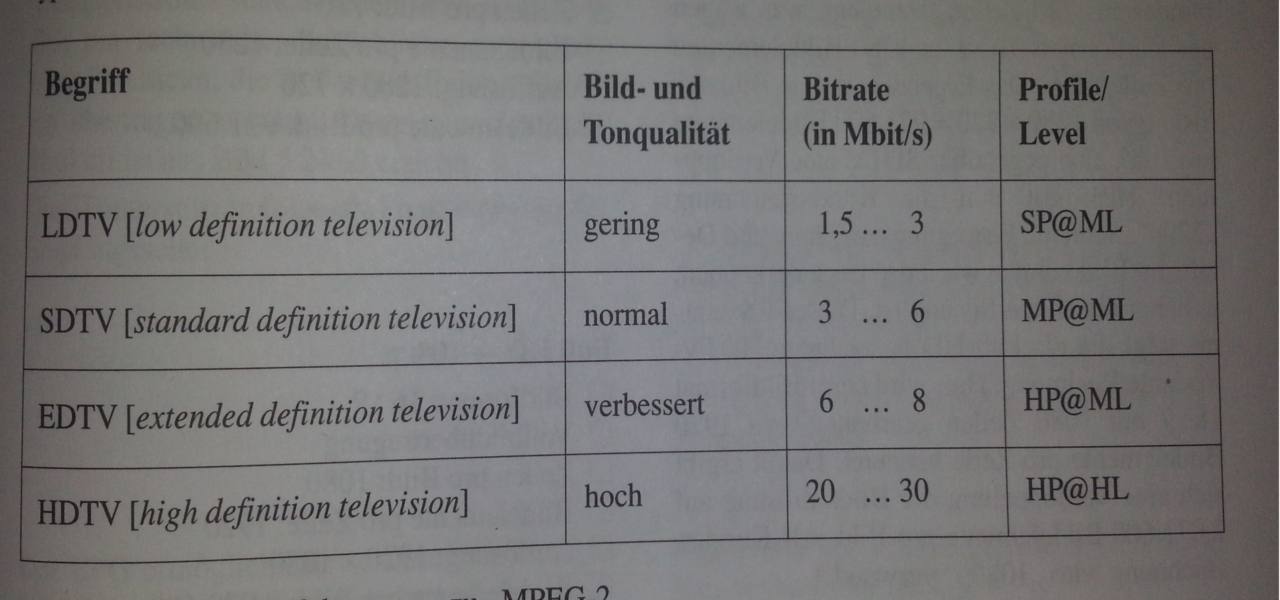
\includegraphics[scale=0.16]{3.png}

\subsubsection{Profile}

Der MPEG2-Standard unterscheidet zwischen fünf verschiedenen Profilen:

\begin{itemize}
\item \textbf{Simple Profile (SP)} $\rightarrow$ ohne bidirektionale Bewegungsschätzung

\item \textbf{Main Profile (MP)} $\rightarrow$ mit bidirektionale Bewegungsschätzung

\item \textbf{SNR (signal-to-noise ratio) / Scaleable Profile (SNRP)} $\rightarrow$  mit Skalierung in Abhängigkeit vom Quantisierungsfehler

\item \textbf{Spatial Scaleable Profile (SSP)} $\rightarrow$ Zusätzliche Skalierung der Bildauflösung

\item \textbf{High Profile (HP)} $\rightarrow$ Alle Skalierungen und Bildformate 16:9

\end{itemize}

\subsubsection{Levels}

Es können zwischen vier verschiedenen Qualitätsstufen unterschieden werden:

\begin{itemize}
\item \textbf{Low Level (LL)} $\rightarrow$ Reduzierte Auflösung

\item \textbf{Main Level (ML)} $\rightarrow$ Standardauflösung

\item \textbf{High-1440-Level (H14L)} $\rightarrow$ Hohe Qualität

\item \textbf{High Level (HL)} $\rightarrow$ Höchste Qualität
\end{itemize}


\subsection{H.264/MPEG4 AVC}

H.264 ist ein Standard zur hocheffizienten Videokompression, der speziell heutzutage bei HDTV verwendet wird. Das Ziel des H.264 Projektes war, ein Kompressionsverfahren zu entwickeln das im Vergleich zu den vorherigen Standards die benötigte Datenrate bei gleicher Qualität mindestens um die Hälfte reduziert.

\end{document}